\documentclass[10pt,twocolumn,letterpaper]{article}
% Formato tipo IEEE (dos columnas, Times 10 pt) sin IEEEtran.cls, que no está instalada.
\usepackage[utf8]{inputenc}
\usepackage[T1]{fontenc}
\usepackage{mathptmx}
\usepackage[letterpaper,top=0.75in,bottom=1in,left=0.625in,right=0.625in,columnsep=0.25in]{geometry}
\usepackage{amsmath,amssymb}
\usepackage{graphicx}
\usepackage{booktabs}
\usepackage{array}
\usepackage{xcolor}
\usepackage{tikz}
\usetikzlibrary{arrows.meta,positioning,fit}
\usepackage[font=footnotesize,labelsep=period]{caption}
\usepackage{titlesec}
\usepackage{cite}
\usepackage{url}
\usepackage{microtype}
\usepackage[hidelinks]{hyperref}

% Sin patrones de guionado en castellano en esta instalación: se evita cortar palabras.
\hyphenpenalty=5000
\exhyphenpenalty=5000
\emergencystretch=1.5em

% Estilo de secciones IEEE
\renewcommand{\thesection}{\Roman{section}}
\renewcommand{\thesubsection}{\Alph{subsection}}
\titleformat{\section}{\normalfont\scshape\centering}{\thesection.}{0.5em}{}
\titlespacing*{\section}{0pt}{1.2ex plus .3ex}{0.8ex}
\titleformat{\subsection}{\normalfont\itshape}{\thesubsection.}{0.5em}{}
\titlespacing*{\subsection}{0pt}{0.9ex plus .2ex}{0.5ex}
\renewcommand{\figurename}{Fig.}
\renewcommand{\tablename}{Tabla}
\renewcommand{\thetable}{\Roman{table}}
\renewcommand{\refname}{Referencias}
\renewcommand{\abstractname}{Resumen}
\setlength{\textfloatsep}{8pt plus 2pt minus 2pt}
\setlength{\floatsep}{6pt plus 2pt minus 2pt}
\captionsetup{skip=4pt}

% Colores comunes a los esquemas
\colorlet{ok}{green!45}
\colorlet{mb}{red!70}
\colorlet{deriva}{green!18}

\title{\Large Menos \emph{macroblocking} en video en vivo sobre SRT:\\ I-headers entregados por el edge}
\author{Vicente Andrade Ercilla\\
\small Estudiante de Ciencias de la Ingeniería Electrónica\\
\small Departamento de Electrónica, Universidad Técnica Federico Santa María, Valparaíso, Chile\\
\small \texttt{vicente.andrade@usm.cl}}
\date{}

\begin{document}
\maketitle

\begin{abstract}
\noindent En video en vivo sobre UDP (\emph{User Datagram Protocol}), un paquete perdido produce \emph{macroblocking}: bloques corruptos que se propagan hasta el próximo cuadro intra, hasta 3~s después con un GoP (\emph{Group of Pictures}) de 90 cuadros. SRT (\emph{Secure Reliable Transport}) retransmite, pero solo dentro de su latencia; lo que no llega a tiempo se descarta. Proponemos que el edge, el servidor que reparte el video, reutilice los I-headers de AGiLE, copias intra de algunos P que ya viajan en el stream, y los entregue solo al espectador que descartó paquetes. No se pide nada al codificador ni se agrega latencia. El edge detecta el descarte con la marca de tiempo de los ACK (\emph{acknowledgement}) de SRT. En un emulador, con la latencia por defecto de SRT, el I-header reduce a la mitad la duración del \emph{macroblocking} en los cortes que SRT no recupera (de 1,1 a 0,5~s por evento). El costo es un 68~\% más de tasa entre el codificador y el edge, una deriva leve después de recuperar y un peor resultado con cortes cortos, que SRT ya cubre.
\end{abstract}

\noindent\textbf{\small Palabras clave:} \small H.264, SRT, pérdida de paquetes, \emph{macroblocking}, edge, GoP.
\normalsize

\section{Introducción}

En video en vivo, el codificador intercala cuadros intra (I), que se decodifican solos, y cuadros predichos (P), que solo describen lo que cambió respecto del anterior. Un GoP largo ahorra bits, pero si se pierde un paquete, el error se copia de P en P hasta el próximo intra y el espectador ve \emph{macroblocking}. Sobre TCP (\emph{Transmission Control Protocol}) la pérdida se convierte en pausas; este trabajo trata el transporte sobre UDP, que se usa cuando importa la latencia.

SRT~\cite{srt} retransmite lo perdido, pero entrega cada paquete con una latencia fija $L$. Si un corte de la red dura más que $L$, el paquete se descarta y el \emph{macroblocking} vuelve. Las salidas conocidas le cobran a todos los espectadores: subir $L$ retrasa a todos, acortar el GoP sube la tasa de todos y pedirle un intra al codificador con un PLI (\emph{Picture Loss Indication}) se lo envía a todos.

AGiLE~\cite{agile} envía al edge, cada cierto número de P, un I-header: el mismo P codificado además como intra, dentro de una SEI (\emph{Supplemental Enhancement Information}). Lo usa para que quien entra al canal no espere el próximo intra. Para el resto, ese I-header ya está en el edge y se descarta.

\textbf{Objetivo.} Que el espectador que perdió paquetes salga del \emph{macroblocking} en el próximo I-header, sin pedir nada al codificador, sin agregar latencia y sin cambiar lo que recibe el espectador sin pérdidas. Las contribuciones son tres:
\begin{enumerate}
\item El edge le entrega el I-header solo al espectador que descartó paquetes (Sección~\ref{sec:metodo}).
\item Una regla para que el emisor SRT sepa qué descartó el receptor, solo con la marca de tiempo de los ACK (\emph{acknowledgement}) (Sección~\ref{sec:deteccion}).
\item Un emulador en C++ con un núcleo portable al STM32N6 y una comparación de UDP y SRT con y sin I-header, que incluye lo que cuesta el I-header (Sección~\ref{sec:resultados}).
\end{enumerate}
La Sección~\ref{sec:previos} resume lo necesario de H.264 y SRT, y la Sección~\ref{sec:relacionados} los trabajos relacionados. La Sección~\ref{sec:problema} plantea el problema, la Sección~\ref{sec:metodo} la estrategia y la arquitectura, la Sección~\ref{sec:resultados} los resultados y la Sección~\ref{sec:conclusiones} las conclusiones.

\section{Antecedentes}
\label{sec:previos}

\subsection{H.264}
En H.264~\cite{h264}, cada imagen se divide en macrobloques de $16\times16$ píxeles, agrupados en \emph{slices}, y cada slice viaja en una NAL (\emph{Network Abstraction Layer unit}). Un P copia cada macrobloque desde el cuadro anterior, desplazado según un vector de movimiento; si ese cuadro está dañado, la copia también. Un IDR (\emph{Instantaneous Decoding Refresh}) es un intra que además vacía las referencias del decodificador. El I-header de AGiLE~\cite{agile} es un intra no-IDR guardado en una SEI de datos de usuario, que el decodificador ignora si no la conoce. La SEI \emph{recovery point} le indica al decodificador que puede retomar desde ese intra.

\subsection{SRT en modo \emph{live}}
El video viaja en paquetes TS (\emph{Transport Stream} de MPEG, \emph{Moving Picture Experts Group}) de 188~B, siete por cada paquete SRT. El receptor de SRT~\cite{srt} avisa cada hueco de inmediato con un NAK (\emph{negative acknowledgement}) y lo repite periódicamente; el emisor retransmite con prioridad. Cada 10~ms, el receptor envía un ACK con el primer paquete que le falta. TSBPD (\emph{Timestamp-Based Packet Delivery}) entrega cada paquete a la aplicación en su marca de tiempo más $L$, que por defecto es de 120~ms~\cite{srt}. Si un paquete todavía falta en ese momento, TLPKTDROP (\emph{Too-Late Packet Drop}) lo salta y el ACK siguiente lo cubre como si hubiera llegado. Según el borrador, el emisor no se entera de ese salto~\cite{srt}.

\section{Trabajos relacionados}
\label{sec:relacionados}

\textbf{AGiLE}~\cite{agile} usa un GoP de 10~s con un I-header cada 2~s, que el edge solo entrega a quien entra al canal. Frente a un GoP fijo de 2~s, logra un BD-rate (\emph{Bjøntegaard Delta rate}, diferencia promedio de bits a igual calidad) de $-3{,}5$~\%. Entrar por un I-header cuesta 1,1~puntos de VMAF (\emph{Video Multimethod Assessment Fusion}), porque los P siguientes se calcularon sobre el P y no sobre el I-header. AGiLE no trata las pérdidas.

\textbf{\emph{Keyframe injection}}~\cite{vanwallendael2021,mareen2024} mantiene un flujo aparte de intras, del que el reproductor pide uno al entrar o al perder paquetes, con una caída menor que 0,94~puntos de VMAF~\cite{vanwallendael2021}. El estudio se extendió a tres generaciones de estándares de video~\cite{mareen2024}, y una versión posterior repara con un P apoyado en un cuadro anterior a la pérdida, para evitar picos de tasa~\cite{mareen2023}.

\textbf{FrameTrace}~\cite{frametrace} mide en Media over QUIC la fracción de cuadros que se muestran. Con 1~\% de pérdida informa VMAF~72,6 con GoP de 0,5~s y 55,7 con GoP de 2~s, y acorta el GoP cuando hay pérdida, lo que exige un lazo hasta el codificador, igual que el PLI de RTP (\emph{Real-time Transport Protocol}).

En los trabajos revisados, la reparación sale de un flujo aparte o de un pedido al codificador. Aquí sale de un intra que ya está en el edge, y la decisión la toma el edge, sin un pedido del reproductor.

\section{Problema}
\label{sec:problema}

Sean $t_0$ el instante en que el edge envía un paquete, $d$ el retardo de ida y $D$ la duración de un corte. El receptor solo puede pedir el paquete cuando el corte termina, y la retransmisión debe llegar antes del plazo $t_0+d+L$. En primera aproximación, SRT recupera el corte si
\begin{equation}
D + \mathrm{RTT} + d \;\lesssim\; L ,
\label{eq:cond}
\end{equation}
donde RTT es el tiempo de ida y vuelta. Con $L=120$~ms, $d=15$~ms y $\mathrm{RTT}=30$~ms, SRT recupera cortes de hasta unos 75~ms. Haivision recomienda $L$ entre 3 y 6~RTT para pérdidas de hasta 7~\%~\cite{haivision}, es decir, de 90 a 180~ms en este caso. Sea cual sea $L$, los cortes más largos que $L-\mathrm{RTT}-d$ se descartan: el slice llega truncado y el \emph{macroblocking} dura hasta el próximo intra (Fig.~\ref{fig:problema}).

\begin{figure}[t]
\centering
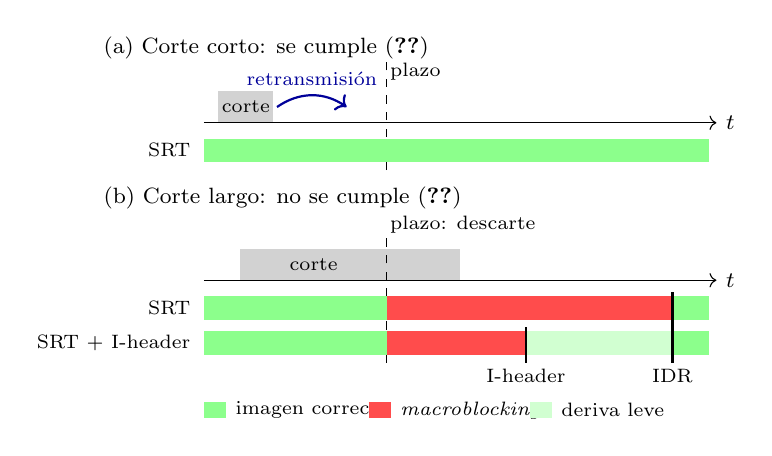
\begin{tikzpicture}[font=\footnotesize, x=0.93cm, y=1cm]
% (a) corte corto
\node[anchor=west] at (0,0.95) {(a) Corte corto: se cumple~\eqref{eq:cond}};
\fill[gray!35] (1.7,0) rectangle (2.45,0.4);
\node[font=\scriptsize] at (2.075,0.2) {corte};
\draw[->] (1.5,0) -- (8.5,0) node[right]{$t$};
\draw[dashed] (4.0,-0.6) -- (4.0,0.8) node[anchor=north west, inner sep=1pt, font=\scriptsize]{plazo};
\draw[->, thick, blue!60!black] (2.5,0.2) to[bend left=35] node[above, font=\scriptsize]{retransmisión} (3.45,0.2);
\fill[ok] (1.5,-0.5) rectangle (8.4,-0.2);
\node[anchor=east, font=\scriptsize] at (1.45,-0.35) {SRT};
% (b) corte largo
\node[anchor=west] at (0,-0.95) {(b) Corte largo: no se cumple~\eqref{eq:cond}};
\fill[gray!35] (2.0,-2.0) rectangle (5.0,-1.6);
\node[font=\scriptsize] at (3.0,-1.8) {corte};
\draw[->] (1.5,-2.0) -- (8.5,-2.0) node[right]{$t$};
\draw[dashed] (4.0,-3.05) -- (4.0,-1.45) node[anchor=south west, inner sep=1pt, font=\scriptsize]{plazo: descarte};
\fill[ok] (1.5,-2.5) rectangle (4.0,-2.2);
\fill[mb] (4.0,-2.5) rectangle (7.9,-2.2);
\fill[ok] (7.9,-2.5) rectangle (8.4,-2.2);
\node[anchor=east, font=\scriptsize] at (1.45,-2.35) {SRT};
\fill[ok] (1.5,-2.95) rectangle (4.0,-2.65);
\fill[mb] (4.0,-2.95) rectangle (5.9,-2.65);
\fill[deriva] (5.9,-2.95) rectangle (7.9,-2.65);
\fill[ok] (7.9,-2.95) rectangle (8.4,-2.65);
\node[anchor=east, font=\scriptsize] at (1.45,-2.8) {SRT + I-header};
\draw[thick] (5.9,-3.05) -- (5.9,-2.6);
\node[font=\scriptsize, below] at (5.9,-3.0) {I-header};
\draw[thick] (7.9,-3.05) -- (7.9,-2.15);
\node[font=\scriptsize, below] at (7.9,-3.0) {IDR};
% leyenda
\fill[ok] (1.5,-3.75) rectangle (1.8,-3.55); \node[anchor=west, font=\scriptsize] at (1.8,-3.65) {imagen correcta};
\fill[mb] (3.75,-3.75) rectangle (4.05,-3.55); \node[anchor=west, font=\scriptsize] at (4.05,-3.65) {\emph{macroblocking}};
\fill[deriva] (5.95,-3.75) rectangle (6.25,-3.55); \node[anchor=west, font=\scriptsize] at (6.25,-3.65) {deriva leve};
\end{tikzpicture}
\caption{Qué ve el espectador según la duración del corte. La barra gris es el corte de la red y la línea discontinua el plazo de entrega del primer paquete perdido. (a) La retransmisión llega antes del plazo y la imagen no se daña. (b) El paquete se descarta en su plazo. Con SRT solo, el \emph{macroblocking} dura hasta el IDR; con I-header, hasta el primer I-header que el edge entrega después de detectar el descarte, seguido de una deriva leve hasta el IDR.}
\label{fig:problema}
\end{figure}

\textbf{Problema.} Acortar el \emph{macroblocking} de los cortes que SRT no recupera, en el tramo edge--espectador, con tres condiciones: no agregar latencia, no cambiar lo que recibe el espectador sin pérdidas y no pedir nada al codificador por cada pérdida. Suponemos que el tramo codificador--edge no pierde paquetes.

\section{Estrategia y arquitectura}
\label{sec:metodo}

La Fig.~\ref{fig:arq} muestra la arquitectura. El codificador (un STM32N6570-DK, con codificador H.264 por hardware) envía al edge el stream con GoP largo y, cada $n$ P, un I-header dentro de una SEI. El edge abre una conexión SRT con cada espectador. Al espectador sin pérdidas le quita las SEI, así que recibe exactamente el stream original. Cuando detecta que un espectador descartó paquetes, reemplaza el próximo P que tenga I-header por la SEI \emph{recovery point} y el I-header, solo para ese espectador.

\begin{figure}[t]
\centering
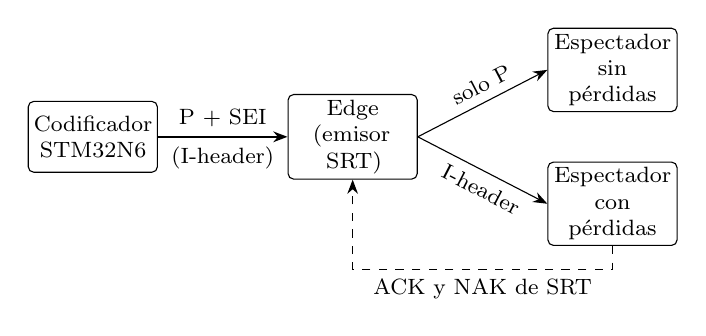
\begin{tikzpicture}[font=\footnotesize,
  box/.style={draw, rounded corners=2pt, align=center, minimum height=9mm, inner sep=2pt, text width=15mm},
  >={Stealth[length=1.8mm]}]
\node[box] (enc) at (0,0) {Codificador\\STM32N6};
\node[box] (edge) at (3.3,0) {Edge\\(emisor SRT)};
\node[box] (v1) at (6.6,0.85) {Espectador\\sin pérdidas};
\node[box] (v2) at (6.6,-0.85) {Espectador\\con pérdidas};
\draw[->, thick] (enc) -- node[above]{P + SEI} node[below]{(I-header)} (edge);
\draw[->] (edge.east) -- node[pos=0.55, above, sloped]{solo P} (v1.west);
\draw[->] (edge.east) -- node[pos=0.55, below, sloped]{I-header} (v2.west);
\draw[->, dashed] (v2.south) -- ++(0,-0.3) -| node[pos=0.25, below]{ACK y NAK de SRT} (edge.south);
\end{tikzpicture}
\caption{Arquitectura. El I-header viaja siempre hasta el edge, que lo entrega solo al espectador que descartó paquetes. El edge lo sabe por los ACK y NAK de SRT, sin un mensaje nuevo.}
\label{fig:arq}
\end{figure}

\begin{figure*}[t]
\centering
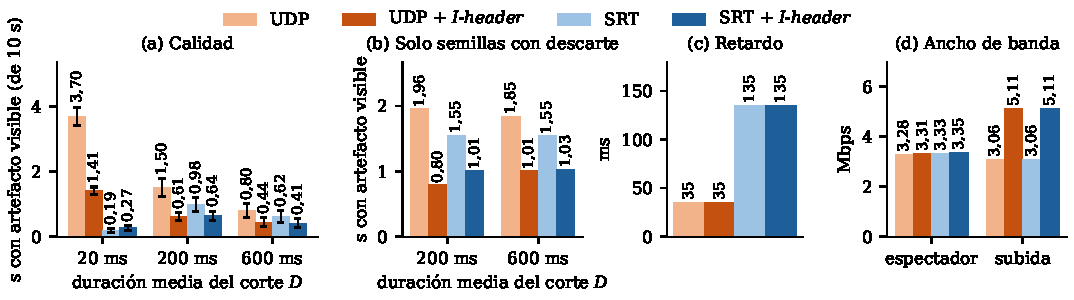
\includegraphics[width=\textwidth]{fig_resultados_gop90.pdf}
\caption{Los cuatro casos con GoP~90 a 30~fps y $L=120$~ms (media de 8 semillas de 10~s). (a) Cuadros con \emph{macroblocking} ($\mathrm{PSNR}_{\mathrm{ref}}<35$~dB) según la duración media del corte $D$, con su error estándar; las barras con flecha están recortadas. (b) Duración media del \emph{macroblocking} por evento, en las semillas donde el caso sin I-header tuvo \emph{macroblocking} (7 con UDP y 4 con SRT para $D=200$~ms; 3 y 3 para $D=600$~ms). (c) Retardo extremo a extremo fijado en el emulador. (d) Tasa hacia el espectador ($D=200$~ms) y tasa de subida codificador--edge.}
\label{fig:res90}
\end{figure*}

\subsection{Cómo detecta el edge el descarte}
\label{sec:deteccion}
El edge no recibe aviso del descarte, pero lo puede inferir. El receptor envía un ACK cada $T_{\mathrm{ACK}}=10$~ms, y si salta un paquete, el ACK siguiente lo cubre igual. Ese ACK lleva la marca de tiempo de cuando se generó~\cite{srt}. Un paquete $s$ que el edge vio en un NAK se descartó si el primer ACK que lo cubre se generó después de su plazo y después de cuando se habría confirmado su última retransmisión:
\begin{equation}
g_s > \max\big(\tau_s,\; r_s + d + T_{\mathrm{ACK}}\big),
\label{eq:regla}
\end{equation}
donde $g_s$ es el instante de generación de ese ACK, $\tau_s=t_{0,s}+d+L$ el plazo de $s$ y $r_s$ el instante de su última retransmisión (si no hubo, solo cuenta $\tau_s$). El segundo término evita marcar un paquete recuperado justo antes de su plazo. La regla supone que el edge no envía retransmisiones que ya no llegarían a tiempo.

\subsection{Generación del I-header}
\label{sec:ih}
En el STM32N6, la API (\emph{Application Programming Interface}) del codificador permite pedir un intra no-IDR y fijar su QP (parámetro de cuantización). En el PC, libx264 no emite intras no-IDR sin cuadros B, así que el núcleo reescribe el encabezado de un IDR como intra no-IDR con el número de cuadro del P que reemplaza. El I-header debe tener el QP de ese P: con un I-header de calidad fija, la deriva fue grande donde el codificador tenía pocos bits.

\subsection{Emulador y métricas}
El núcleo (C++17, sin memoria dinámica ni dependencias del sistema operativo) lee el H.264, arma la SEI, reescribe el encabezado y genera el TS; es la parte que correrá en el STM32N6, separada de la HAL (\emph{Hardware Abstraction Layer}). En el PC, un simulador de eventos discretos modela SRT en modo \emph{live} según el borrador~\cite{srt}. El canal alterna entre un estado bueno y cortes sin entrega de duración media $D$ (modelo de Gilbert--Elliott) y depende solo del tiempo y de una semilla, así que todos los casos ven los mismos cortes. Sin pérdida, el video decodificado es idéntico bit a bit al original.

La calidad de cada cuadro $k$ se mide con el PSNR (\emph{Peak Signal-to-Noise Ratio}) de la luminancia, a partir del error cuadrático medio (MSE, \emph{Mean Squared Error}) entre la imagen de referencia $Y_k$ y la recibida $\hat Y_k$, de $W\times H$ píxeles de 8 bits:
\begin{equation}
\mathrm{PSNR}_k=10\log_{10}\frac{255^2}{\frac{1}{WH}\sum_{i,j}\big(Y_k(i,j)-\hat Y_k(i,j)\big)^2}\ \ \mathrm{[dB]}.
\end{equation}
El ``ruido'' es la diferencia píxel a píxel. $\mathrm{PSNR}_{\mathrm{ref}}$ compara con el mismo stream decodificado sin pérdida, así que solo mide lo que agregan la pérdida y la deriva. $\mathrm{PSNR}_{\mathrm{fuente}}$ compara con el video crudo. Un cuadro tiene \emph{macroblocking} si $\mathrm{PSNR}_{\mathrm{ref}}<35$~dB, umbral elegido por nosotros. Un cuadro que no llega se reemplaza por el anterior. VMAF estima la calidad percibida (0 a 100) con un modelo entrenado con notas de observadores; todavía no lo medimos.

\section{Resultados}
\label{sec:resultados}


\textbf{Configuración.} Los primeros 300 cuadros de un clip, a $1280\times720$ y 30~fps, codificados con libx264 en perfil Baseline a 3~Mbps, con 45 slices por cuadro y GoP~90. Hay un I-header cada 5 P, con el QP del P que reemplaza. El retardo de ida es de 15~ms; SRT usa $L=120$~ms y, sin SRT, el espectador tiene un búfer de 20~ms. Elegimos cortes a ambos lados de~\eqref{eq:cond}: de 20~ms (2~\% del tiempo), que caben en $L$, y de 200 y 600~ms (4~\%), que no caben. No afirmamos con qué frecuencia ocurren estos cortes en una red real. Con UDP + I-header, el espectador avisa cada descarte; con SRT + I-header, el edge usa la regla~\eqref{eq:regla}.

\subsection{Calidad, latencia y ancho de banda}
La Fig.~\ref{fig:res90} compara los cuatro casos. Sin retransmisión, el I-header reduce los cuadros con \emph{macroblocking} a la mitad o menos con los tres tipos de corte. Con cortes de 20~ms, SRT solo deja 5,2 cuadros con \emph{macroblocking}, y agregar el I-header lo empeora a 15,8: empeoró en 2 de las 8 semillas y mejoró en 1. Con cortes de 200 y 600~ms, SRT no recupera el corte en 4 y 3 de las 8 semillas. En esos eventos, el I-header baja la duración del \emph{macroblocking} de 1,12 a 0,54~s y de 1,08 a 0,51~s. Con cortes de 600~ms, SRT no mejora a UDP.

El I-header no agrega retardo. La alternativa es subir $L$: con 250~ms desaparecen los eventos de 200~ms, pero los de 600~ms requieren 1000~ms, y ese retardo lo pagan todos los espectadores. La tasa hacia el espectador crece 0,3~\% frente a SRT, porque el I-header solo baja cuando hay pérdida.

\subsection{Qué perdemos}
La Tabla~\ref{tab:costos} resume el costo del I-header. El mayor es la subida: un I-header cada 5 P lleva la tasa codificador--edge de 3,1 a 5,2~Mbps, aunque se paga una vez y no por espectador. Después de recuperar, el espectador no vuelve a la imagen exacta hasta el IDR. Para medir esa deriva sola, se forzó un I-header sin pérdida en 10 cuadros. Con QP cercano a 29, el $\mathrm{PSNR}_{\mathrm{ref}}$ no bajó de 39,3~dB; con QP de 39 a 44, bajó a 28--35~dB. Contra la fuente, la diferencia fue de 1,0 a 1,4~dB.

\begin{table}[t]
\centering
\caption{Costo del I-header con GoP~90, frente al mismo caso sin I-header.}
\label{tab:costos}
\footnotesize
\setlength{\tabcolsep}{4pt}
\begin{tabular}{@{}l>{\raggedright\arraybackslash}p{40mm}@{}}
\toprule
Costo & Valor \\
\midrule
Tasa codificador--edge & $+68$~\% (de 3,1 a 5,2 Mbps) \\
Tasa hacia el espectador & $+0{,}3$~\% (SRT, $D=200$ ms) \\
Retardo agregado & 0 \\
Deriva hasta el IDR & $\mathrm{PSNR}_{\mathrm{ref}}\ge39{,}3$~dB con QP $\approx29$; 28--35~dB con QP 39--44; de $-1{,}0$ a $-1{,}4$~dB contra la fuente \\
Cortes cortos ($D=20$ ms) & de 5,2 a 15,8 cuadros con \emph{macroblocking} \\
Espera hasta recuperar & 0,5~s por evento ($D=200$ y 600 ms) \\
Pico de tasa al enviar el I-header & no medido \\
Cómputo en codificador y edge & no medido \\
\bottomrule
\end{tabular}
\end{table}

\subsection{Validez}
Estos resultados tienen cuatro límites. Primero, son pocos eventos: 7 cortes no recuperados por SRT en 16 corridas de 10~s, con un solo clip. Segundo, el modelo de SRT no está validado contra libsrt y supone que el edge conoce sin error el instante de generación del ACK. Tercero, $L=120$~ms queda bajo la recomendación de Haivision para 4~\% de pérdida (180~ms)~\cite{haivision}, aunque con 180~ms los cortes de 200 y 600~ms tampoco cumplen~\eqref{eq:cond}. Cuarto, el umbral de 35~dB cuenta como \emph{macroblocking} también la deriva fuerte del I-header, que no es un artefacto de bloques; separarlos requiere una métrica perceptual como VMAF.

\section{Conclusiones y trabajo futuro}
\label{sec:conclusiones}
SRT no elimina el \emph{macroblocking}: quedan los cortes más largos que $L-\mathrm{RTT}-d$. En esos cortes, el I-header que ya está en el edge redujo a la mitad la duración del \emph{macroblocking}, sin agregar latencia y con 0,3~\% más de tasa hacia el espectador. El edge sabe a quién enviarlo sin cambiar SRT, por la marca de tiempo de los ACK. El costo está en la subida (+68~\%) y en una deriva hasta el IDR. Con cortes cortos SRT basta y el I-header empeora el resultado, así que el edge debe enviarlo solo cuando el descarte es largo.

Como trabajo futuro quedan:
(i) la misma comparación con GoP~30;
(ii) más eventos, varios clips y la $L$ recomendada;
(iii) medir VMAF para separar deriva de \emph{macroblocking};
(iv) una política del edge que no envíe el I-header con cortes cortos, con QP alto o con el IDR cerca;
(v) validar el modelo contra libsrt sobre una red emulada;
(vi) llevar el núcleo al STM32N6.

\begin{thebibliography}{9}
\footnotesize
\setlength{\itemsep}{1pt}
\bibitem{srt} M.~P.~Sharabayko, M.~A.~Sharabayko, J.~Dube, J.~S.~Kim y J.~W.~Kim, ``The SRT protocol,'' IETF Internet-Draft draft-sharabayko-srt-01, trabajo en curso, 2021. [En línea]. Disponible: \url{https://datatracker.ietf.org/doc/draft-sharabayko-srt/}
\bibitem{agile} C.~Chen, W.~Yin, Z.~Huang y S.~Shi, ``AGiLE: Enhancing adaptive GOP in live video streaming,'' en \emph{Proc. ACM Multimedia Systems Conf. (MMSys '24)}, 2024, pp.~34--44, doi: 10.1145/3625468.3647609.
\bibitem{h264} ITU-T, ``Advanced video coding for generic audiovisual services,'' Recomendación ITU-T H.264, ago. 2024. [En línea]. Disponible: \url{https://www.itu.int/rec/T-REC-H.264}
\bibitem{vanwallendael2021} G.~Van~Wallendael, H.~Mareen, J.~Vounckx y P.~Lambert, ``Keyframe insertion: Enabling low-latency random access and packet loss repair,'' \emph{Electronics}, vol.~10, no.~6, art.~748, 2021, doi: 10.3390/electronics10060748.
\bibitem{mareen2024} H.~Mareen, M.~Courteaux, P.-J. Speelmans, P.~Lambert y G.~Van~Wallendael, ``A study on keyframe injection in three generations of video coding standards for fast channel switching and packet-loss repair,'' \emph{Multimedia Tools and Applications}, vol.~83, pp.~44485--44501, 2024, doi: 10.1007/s11042-023-17163-2.
\bibitem{mareen2023} H.~Mareen, P.~Lambert y G.~Van~Wallendael, ``P-frame injection for efficient packet-loss repair in ultra-low-latency video streaming,'' en \emph{Proc. IEEE Int. Conf. Visual Communications and Image Processing (VCIP)}, 2023. [En línea]. Disponible: \url{https://ieeexplore.ieee.org/document/10402720/}
\bibitem{frametrace} B.~Denizer, L.~Winkel y O.~Landsiedel, ``FrameTrace: Frame-level telemetry for Media over QUIC,'' en \emph{Proc. EMS '25, ACM SIGCOMM 2025 Workshops}, 2025, pp.~31--36, doi: 10.1145/3746441.3748231.
\bibitem{haivision} Haivision, ``SRT latency,'' en \emph{SRT Protocol Documentation}, v1.5.3. [En línea]. Disponible: \url{https://doc.haivision.com/SRT/1.5.3/Haivision/latency}
\end{thebibliography}

\end{document}
